\section{Addierer (Konstante)}
\label{sec:knf:konstadd}

Für die Addition der Rundenkonstanten wird eine Addition konstruiert, die Literale für die Konstanten vermeidet.
Da die Konstanten bekannt sind, können der Halbaddierer, der Volladdierer und der Mod-2 Addierer entsprechend reduziert werden.
Abbildung \ref{fig:adder_reduced} zeigt die reduzierten Varianten. In der ersten Zeile der Tabelle sind die Varianten dargestellt,
die genutzt werden, falls das eigehende Bit (b) der Konstante den Wert $0$ hat. Entsprechend sind in der zweiten Zeile die Varianten für ein
Bit (b) mit dem Wert $1$ dargestellt.
\begin{figure}[!h]
  \centering
  \begin{tabular}{r|c|c|c}
    \hiderowcolors
    b & Halbaddierer                                 & Volladdierer                                 & Mod-2 Addierer\\
    \hline
    0 & \begin{minipage}{0.29\textwidth}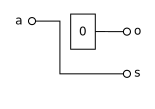
\includegraphics[scale=1]{images/halfadder0}\end{minipage} & \begin{minipage}{0.29\textwidth}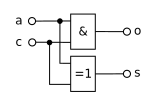
\includegraphics[scale=1]{images/fulladder0}\end{minipage} & \begin{minipage}{0.29\textwidth}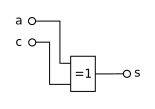
\includegraphics[scale=1]{images/lastadder0}\end{minipage}\\
    \hline
    1 & \begin{minipage}{0.29\textwidth}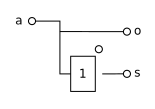
\includegraphics[scale=1]{images/halfadder1}\end{minipage} & \begin{minipage}{0.29\textwidth}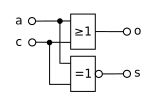
\includegraphics[scale=1]{images/fulladder1}\end{minipage} & \begin{minipage}{0.29\textwidth}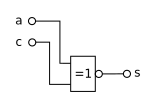
\includegraphics[scale=1]{images/lastadder1}\end{minipage}\\
    \showrowcolors
  \end{tabular}
  \caption[Reduziert Addierer]{Reduzierte Addierer\protect\footnotemark}
  \label{fig:adder_reduced}
\end{figure}
\footnotetext{Jeweils auf Basis von MovGP0, CC BY-SA 2.0 de, \url{https://commons.wikimedia.org/w/index.php?curid=22912775}}

Ein Halbaddierer der zwei Bits addiert und am Eingang (b) den Wert $0$ erhält, gibt den Wert des Eingangs (a) direkt an die Summe (s) weiter.
Der Übertrag (o) kann dabei niemals $1$ werden. Hat der Eingang (b) den Wert $1$, liegt immer genau dann ein Übertrag (o) vor, wenn am Eingang (a)
der Wert $1$ anliegt. Die Summe (s) hat jedoch nur den Wert $1$, falls der Wert $0$ am Eingang (a) anliegt. Der Eingang (a) muss invertiert werden.

Der Volladdierer addiert drei Bits. Liegt dabei an einem beliebigen Eingang ein Bit mit dem Wert $0$ an, brauchen nur noch zwei Bits addiert werden.
Der Volladdierer kann auf einen Halbaddierer reduziert werden. Liegt am Eingang (b) der Wert $1$ an, ist für einen Übertrag nur noch Vorraussetzung,
das Eingang (a) oder Übertrag (c) den Wert $1$ haben. Für die Summe (s) liegt durch den Eingang (b) schon ein $1$-Bit vor. Die Summe (s) ist nur dann
$1$, wenn der Eingang(a) und der Übertrag (c) gleich sind, was sich durch den inversen XOR-Operator beschreiben lässt.

Die Mod-2 Addierer werden, wie schon in Abschnitt \ref{sec:grundlagen_add} durchgeführt, aus den Volladdierern erzeugt, indem die für den Übertrag
notwendigen Operatoren entfernt werden.

Nach der Erstellung der reduzierten Addierer, werden die konjunktiven Normalformen erstellt. Wie auch im vorhergehenden Abschnitt werden zwei mögliche
Lösungen generiert, um eine optimale Lösung sowohl mit, als auch ohne XOR-Unterstützung bereit zu stellen. eqntott und Espresso werden dabei nur mit
einbezogen, falls der Übertrag und die Summe in Abhängigkeit von den selben Literalen berechnet werden. Im anderen Fall lässt sich die optimale Lösung
direkt durch die Verwendung der Gatter generieren.

Die Summe und der Übertrag bei einem Halbaddierer mit eingehendem Bit (b) = $1$ werden beide in Abhängigkeit des Eingangs (a) berechnet. Die boolsche
Gleichung in Abbildung \ref{fig:halfadder1_qen} wird deshalb genutzt um eine optimale konjunktive Normaform zu berechnen. Für den anderen Fall ergibt
sich die optimale Lösung direkt aus der Anwendung der Gatter.
\begin{figure}[!h]
  \centering
  \begin{lstlisting}[]
  NAME = HalfAdderConst1;
  INORDER = c_out s_out a_in;
  OUTORDER = z;

  z = eq(c_out, a_in) & eq(s_out, !a_in);
  \end{lstlisting}
  \caption{Halbaddierer (1) - Gleichung}
  \label{fig:halfadder1_qen}
\end{figure}

Abbildung \ref{fig:red_halfadder_cnf} zeigt die ermittelten konjunktiven Normalformen. Unabhängig von dem eigehenden Bit (b) sind bei der Unterstützung
von XOR-Klauseln zwei Klauseln notwendig, während es im anderen Fall drei Klauseln sind. Bei Verwendung der Gatter sind die Klauseln entsprechend beschriftet.
Eine Umwandlung der XOR-Klauseln in normale Klauseln führt für den Fall des eigenenden Bits (b) = 0 ebenfalls zu drei Klauseln während es im anderen Fall vier
Klauseln sind.
\begin{figure}[!h]
  \centering
  \begin{minipage}[c]{0.3cm}
    ~
  \end{minipage}
  \begin{minipage}[c]{7.1cm}
    ~~~~~~~~~~~~~~~~~~~~~~~~~~~~~~~b = $0$
  \end{minipage}
  \begin{minipage}[c]{7cm}
    ~~~~~~~~~~~~~~~~~~~~~~~~~~~~~~~b = $1$
  \end{minipage}
  \begin{minipage}[l]{0.4cm}
    ~
  \end{minipage}
  \begin{minipage}[l]{3.5cm}
    \underline{Ohne XOR}\\
    ~\\
    \underline{Übertrag - $0$}\\
    $ (\overline{o}) ~ \wedge $\\
    \underline{Summe - EQ}\\
    $ (\overline{s} \vee  a) ~ \wedge $\\
    $ (s \vee \overline{a}) $
  \end{minipage}
  \begin{minipage}[l]{3.5cm}
    \underline{Mit XOR}\\
    ~\\
    \underline{Übertrag - $0$}\\
    $ (\overline{o}) ~ \wedge $\\
    \underline{Summe - EQ}\\
    $ (\overline{s} \veebar a) $\\
    ~
  \end{minipage}
  \begin{minipage}[l]{3.5cm}
    \underline{Ohne XOR}\\
    ~\\
    $ (o \vee  s) ~ \wedge $\\
    $ (\overline{s} \vee  \overline{a}) ~ \wedge $\\
    $ (\overline{o} \vee  a) $\\
    ~\\
    ~
  \end{minipage}
  \begin{minipage}[l]{3.5cm}
    \underline{Mit XOR}\\
    ~\\
    \underline{Übertrag - EQ}\\
    $ (\overline{o} \veebar a) ~ \wedge $\\
    \underline{Summe - NOT}\\
    $ (s \veebar a) $\\
    ~
  \end{minipage}
  \caption{Reduzierter Halbaddierer - Konjuktive Normalform}
  \label{fig:red_halfadder_cnf}
\end{figure}

Ein Volladdierer mit eingehendem Bit (b) = 0 entspricht exakt einem Halbaddierer. Die konjunktive Normalform wird für diesen Fall direkt übernommen.
Im anderen Fall dient die boolsche Gleichung in Abbildung \ref{fig:fulladder1_qen} zur Ermittlung der konjunktiven Normalform.
\begin{figure}[!h]
  \centering
  \begin{lstlisting}[]
  NAME = FullAdderConst1;
  INORDER = c_out s_out a_in c_in;
  OUTORDER = z;

  z = eq(c_out, a_in | c_in) & eq(!s_out, xor(c_in, a_in));
  \end{lstlisting}
  \caption{Volladdierer (1) - Gleichung}
  \label{fig:fulladder1_qen}
\end{figure}

Die konjunktiven Normalformen für den Volladdierer sind in Abbildung \ref{fig:red_halfadder_cnf} aufgeführt. Wie auch bei dem Halbaddierer ist die Anzahl
der Klauseln unabhängig von dem eigehenden Bit (b). Bei einer Unterstützung von XOR-Klauseln sind vier Klauseln notwendig während es ohne Unterstützung
sechs Klauseln sind. Eine Umwandlung der XOR-Klauseln führt in beiden Fällen zu einer Klauselanzahl von sieben.
\begin{figure}[!h]
  \centering
  \begin{minipage}[c]{0.3cm}
    ~
  \end{minipage}
  \begin{minipage}[c]{7.1cm}
    ~~~~~~~~~~~~~~~~~~~~~~~~~~~~~~~b = $0$
  \end{minipage}
  \begin{minipage}[c]{7cm}
    ~~~~~~~~~~~~~~~~~~~~~~~~~~~~~~~b = $1$
  \end{minipage}
  \begin{minipage}[l]{0.4cm}
    ~
  \end{minipage}
  \begin{minipage}[l]{3.5cm}
    \underline{Ohne XOR}\\
    ~\\
    $ (\overline{s} \vee a \vee c) ~ \wedge $\\
    $ (\overline{o} \vee \overline{s}) ~ \wedge $\\
    $ (\overline{o} \vee c) ~ \wedge $\\
    $ (o \vee \overline{a} \vee \overline{c}) ~ \wedge $\\
    $ (s \vee a \vee \overline{c}) ~ \wedge $\\
    $ (s \vee \overline{a} \vee c) $
  \end{minipage}
  \begin{minipage}[l]{3.5cm}
    \underline{Mit XOR}\\
    ~\\
    \underline{Übertrag - AND}\\
    $ (\overline{o} \vee a) ~ \wedge $\\
    $ (\overline{o} \vee c) ~ \wedge $\\
    $ (o \vee \overline{a} \vee \overline{c}) ~ \wedge $\\
    \underline{Summe - XOR}\\
    $ (\overline{s} \veebar a \veebar c) $
  \end{minipage}
  \begin{minipage}[l]{3.5cm}
    \underline{Ohne XOR}\\
    ~\\
    $ (s \vee \overline{a} \vee \overline{c}) ~ \wedge $\\
    $ (o \vee s) ~ \wedge $\\
    $ (o \vee \overline{a}) ~ \wedge $\\
    $ (\overline{s} \vee a \vee \overline{c}) ~ \wedge $\\
    $ (\overline{o} \vee \overline{s} \vee c) ~ \wedge $\\
    $ (\overline{o} \vee a \vee c) $
  \end{minipage}
  \begin{minipage}[l]{3.5cm}
    \underline{Mit XOR}\\
    ~\\
    \underline{Übertrag - OR}\\
    $ (o \vee \overline{a}) ~ \wedge $\\
    $ (o \vee \overline{c}) ~ \wedge $\\
    $ (\overline{o} \vee a \vee c) ~ \wedge $\\
    \underline{Summe - XNOR}\\
    $ (s \veebar a \veebar c) $
  \end{minipage}
  \caption{Reduzierter Volladdierer - Konjuktive Normalform}
  \label{fig:red_fulladder_cnf}
\end{figure}

Für den Mod-2 Addierer brauchen eqntott und Espresso nicht herangezogen werden. Dieser berechnet die Summe direkt durch den XOR-Operator.
Abbildung \ref{fig:red_lastadder_cnf} zeigt die konjunktiven Normalformen für den Mod-2 Addierer. Auch hier hat das eingehende Bit (b)
keinen Einfluss auf die Anzahl der Klauseln. Mit Unterstützung von XOR-Klauseln ist eine einzelne Klausel ausreichend während ohne
Unterstützung vier Klauseln benötigt werden.
\begin{figure}[!h]
  \centering
  \begin{minipage}[c]{0.3cm}
    ~
  \end{minipage}
  \begin{minipage}[c]{7.1cm}
    ~~~~~~~~~~~~~~~~~~~~~~~~~~~~~~~b = $0$
  \end{minipage}
  \begin{minipage}[c]{7cm}
    ~~~~~~~~~~~~~~~~~~~~~~~~~~~~~~~b = $1$
  \end{minipage}
  \begin{minipage}[l]{0.4cm}
    ~
  \end{minipage}
  \begin{minipage}[l]{3.5cm}
    \underline{Ohne XOR}\\
    ~\\
    \underline{Summe - XOR}\\
    $ (\overline{s} \vee \overline{a} \vee \overline{c}) ~ \wedge $\\
    $ (s \vee a \vee \overline{c}) ~ \wedge $\\
    $ (s \vee \overline{a} \vee c) ~ \wedge $\\
    $ (\overline{s} \vee a \vee c) $
  \end{minipage}
  \begin{minipage}[l]{3.5cm}
    \underline{Mit XOR}\\
    ~\\
    \underline{Summe - XOR}\\
    $ (\overline{s} \veebar a \veebar c) $\\
    ~\\
    ~\\
    ~
  \end{minipage}
  \begin{minipage}[l]{3.5cm}
    \underline{Ohne XOR}\\
    ~\\
    \underline{Summe - XNOR}\\
    $ (s \vee \overline{a} \vee \overline{c}) ~ \wedge $\\
    $ (\overline{s} \vee a \vee \overline{c}) ~ \wedge $\\
    $ (\overline{s} \vee \overline{a} \vee c) ~ \wedge $\\
    $ (s \vee a \vee c) $
  \end{minipage}
  \begin{minipage}[l]{3.5cm}
    \underline{Mit XOR}\\
    ~\\
    \underline{Summe - XNOR}\\
    $ (s \veebar a \veebar c) $\\
    ~\\
    ~\\
    ~
  \end{minipage}
  \caption{Reduzierter Mod-2 Addierer - Konjuktive Normalform}
  \label{fig:red_lastadder_cnf}
\end{figure}

Wie auch für den Addierer im vorhergehenden Abschnitt sind in Abbildung \ref{fig:red_add_literalclausecount} noch mal alle Ergebnisse aufgelistet.
Die Daten der gatterbasierten Lösungen entsprechen in diesem Fall den Daten der XOR-basierten Lösungen mit und ohne Unterstützung von XOR-Klauseln,
da sich alle Überträge und Summen mit Hilfe einer Operation direkt aus den Eingangswerten ergeben. Zusätzliche Literale sind nicht notwendig.
\begin{figure}[!h]
  \centering
  \begin{tabular}{l|rrr|r}
    \hiderowcolors
                           & Halbaddierer & Volladdierer & Mod-2 Addierer &    Gesamt \\
    \hline
    Gatter                 &        3 - 4 &        4 - 7 &          3 - 4 & 95 - 218 \\
    Gatter mit XOR         &        3 - 2 &        4 - 4 &          3 - 1 & 95 - 123 \\
    eqntott \& Espresso    &        3 - 3 &        4 - 6 &          3 - 4 & 95 - 187 \\
    XOR                    &        3 - 2 &        4 - 4 &          3 - 1 & 95 - 123 \\
    XOR ohne Unterstützung &        3 - 4 &        4 - 7 &          3 - 4 & 95 - 218 \\
    \showrowcolors
  \end{tabular}
  \caption{Reduzierter Addierer - Literale und Klauseln}
  \label{fig:red_add_literalclausecount}
\end{figure}

Für die Addition von Konstanten ist es ebenfalls sinnvoll zwei Lösungen zu implementieren. Bei der Unterstützung von XOR-Klauseln wird die gatterbasierte
Lösung verwendet während im anderen Fall die Lösung von eqntott und Espresso verwendet wird.